%%%%%%%%%%%%%%%%%%%%%%%%%%%%%%%%%%%%%%%%%%%%%%%%%%%%%%%%%%%%%%%%%%%%%%%%%%%%%
%% MS LDD - Pedro - 19 July 2006
% Revised for 2008
%%%%%%%%%%%%%%%%%%%%%%%%%%%%%%%%%%%%%%%%%%%%%%%%%%%%%%%%%%%%%%%%%%%%%%%%%%%%%
%%%%%%%%%%%%%%%%%%%%%%%%%%%%%%%%%%%%%%%%%%%%%%%%%%%%%%%%%%%%%%%%%%%%% Headers
\documentclass[a4paper,12pt]{article}
\usepackage{amsmath,amssymb}
%\usepackage[utf8]{inputenc}
%\usepackage[applemac]{inputenc}
\usepackage{geometry}
\usepackage{lscape}
\usepackage{setspace}
\usepackage{framed}
\usepackage{verbatim}
\usepackage{graphicx}
\usepackage{epstopdf}
\usepackage{booktabs}
\usepackage{natbib}
\usepackage{longtable}
\usepackage{rotating}                                                          
\newcommand{\tab}{\hspace{5mm}}
\usepackage{tabularx} 
\usepackage[margin=10pt,font=small,labelfont=bf]{caption}
\usepackage[left,pagewise]{lineno}
\usepackage{caption}
\DeclareGraphicsRule{.tif}{png}{.png}{`convert #1 `basename #1 .tif`.png}
\usepackage{fancyhdr} % This should be set AFTER setting up the page geometry
\pagestyle{fancy}     % options: empty , plain , fancy
\renewcommand{\headrulewidth}{0pt} % customise the layout...
\lhead{{\tiny Jordano - LDD events}}\chead{}\rhead{}
\lfoot{}\cfoot{\thepage}\rfoot{}
%%%%%%%%%%%%%%%%%%%%%%%%%%%%%%%%%%%%%%%%%%%%%%%%%%%%%%%%%%%%%%%%%% Title page
\begin{document}
\title{Manuscript Draft\\
\vspace{2cm}
What is long-distance dispersal? and a taxonomy of dispersal events}

\author{Pedro Jordano$^{\dag}$}

\date{Sevilla, \today}
\maketitle


\begin{spacing}{1.0}
$^{\dag}$ {\small Integrative Ecology Group, Estaci\'on Biol\'ogica de 
Do\~nana, CSIC, Pabell\'on del Per\'u, Avda. Mar\'ia Luisa, s/n, 
E-41013 Sevilla, Spain.}\\


{\small \textit{Corresponding author:} Pedro Jordano. Integrative Ecology Group, Estaci\'on Biol\'ogica de Do\~nana, CSIC, Pabell\'on del Per\'u, Avda. Mar\'ia Luisa, s/n, E-41013 Sevilla, Spain. Fax number: +34 95 4621125. Email address: jordano@ebd.csic.es}\\

\textbf{Key words}: dispersal kernel, fragmentation, frugivores, gene-flow, genetic neighborhood, long-distance dispersal, seed dispersal\\

{\small \textbf{Manuscript information: }** Words; ** Chars; ** Pages, * Figures; * Tables.}
\maketitle
\newpage
%%%%%%%%%%%%%%%%%%%%%%%%%%%%%%%%%%%%%%%%%%%%%%%%%%%%%%%%%%%%%%%%%%%% Abstract
\begin{linenumbers}
\section*{Abstract}

Long-distance dispersal (LDD) is a major component of the population dynamics, genetic structure, and biogeographic history of plant species. It determines the colonization ability of new habitats and the possibilities for fragmented populations to sustain a cohesive metapopulation by inmigration-emigration dynamics that rely on LDD events. Yet our current understanding of the extent, frequency, and consequences of LDD is very limited. On one hand, theoretical models fail to predict accurately the behavior of the tail of the dispersal functions, and thus fail to predict very basic properties of LDD. On the other hand, we still have very limited documentation of actual LDD events in natural populations and consider LDD as a sporadic, rarely far-reaching process marked with the stamp of natural history cursiosity. Here we propose an explicit definition of LDD and what constitutes a LDD event. We propose a combination of ecological and genetic evidences to define LDD events. LDD events should be characterized in terms of distance relative to the ecological limits of the population (in a metapopulation context) and to the limits of the genetic neighborhood.

\end{linenumbers}

\end{spacing}

%%%%%%%%%%%%%%%%%%%%%%%%%%%%%%%%%%%%%%%%%%%%%%%%%%%%%%%%%%%%%%%% Introduction
\begin{flushleft}
\begin{spacing}{1.5}
\newpage 
\begin{linenumbers}
\section*{Introduction}

- General overview of LDD events.

- LDD events no so uncommon, especially for animal-mediated dispersal of pollen and seeds, but also for abiotic dispersal when singular events (strong wind uplift, tornadoes, water runoff) occur.

- Despite extensive evidence for the occurrence of LDD events and recents evidences of far-reaching consequences, no unambiguous definition of LDD still available. 

- Adequate definition probably requires transdisciplinary concepts, from landscape ecology, metapopulation ecology and population genetics. Key ingredients to the definition would be landscape connectivity, genetic neighborhood size.

%%%%%%%%%%%%%%%%%%%%%%%%%%%%%%%%%%%%%%%%%%%%%%%%%%%%%%% Materials and Methods
\begin{comment}
\section*{Material and Methods}
\subsection*{ Species and study site characteristics}

The study species, \textit{Prunus mahaleb} (L.) (Rosaceae), is a tree  producing fleshy-fruits ingested by frugivores that disperse  their seeds after regurgitating or defecating them.  

\subsection*{*}

\subsubsection*{Sampling of dispersed seeds}
\end{comment}

%%%%%%%%%%%%%%%%%%%%%%%%%%%%%%%%%%%%%%%%%%%%%%%%%%%%% Results  and Discussion

\section*{Results and Discussion}

\subsection*{Individual and population neighborhoods as reference marks}

- NOTE. Take evidence from Prunus for reliable estimates of percent pollen and seed coming from outside the population, compare estimates of neighbourhood size with e.g. work on Ficus in BCI \citep{E3.2543,Nason:1996,Stacy:1996vo} and Fraxinus \citep{Bacles:2006kq}.

- Population graph approach \citep{Dyer04}.


\subsection*{Evidences of neighborhood sizes and LDD events}

\subsection*{Challenges and promising avenues for research}

%%%%%%%%%%%%%%%%%%%%%%%%%%%%%%%%%%%%%%%%%%%%%%%%%%%%%%%%%%%%%%%%%%%%%%%%%%%%%
\section*{Acknowledgements}

I am indebted to Jos\'e A. Godoy, Manolo Carri\'on, Juan Luis Garc\'ia-Casta\~no, Jes\'us Rodr\'iguez, Cristina Garc\'ia and, especially, Juan Miguel Arroyo for generous help with field and laboratory work and making possible this study. We appreciate the help and advice of Cristina Garc\'ia, Jos\'e A. Godoy and Jordi Bascompte during the final stages of the manuscript. The study was supported by the Spanish Ministerio de Ciencia y Tecnolog\'ia (REN2003-0273 and CGL2006-00373 to PJ). The Agencia de Medio Ambiente, Junta de Andaluc\'ia, provided generous facilities that made possible this study in the Sierra de Cazorla and authorized my work there. 

\newpage
%%%%%%%%%%%%%%%%%%%%%%%%%%%%%%%%%%%%%%%%%%%%%%%%%%%%%%%%%%%%%%%%%% References
%\section{References}
\bibliographystyle{ecology_letters} % Choose EcolLett style for bibliography
%\bibliography{/Users/pedro/Documents/Databases/Bib_database}
\bibliography{MS_LDD}
%%%%%%%%%%%%%%%%%%%%%%%%%%%%%%%%%%%%%%%%%%%%%%%%%%%%%%%%%%%%%%%%%%%%%%%%%%%%%%
\end{linenumbers}

\end{spacing}

\end{flushleft}
%%%%%%%%%%%%%%%%%%%%%%%%%%%%%%%%%%%%%%%%%%%%%%%%%%%%%%%%%%%%%%%%%%%%%%%%%%%%%
%:----MS NOTES
\begin{comment}

Breeding unit size. Donor number is related to the size of the breeding unit (N individuals) as d= Np, where d is the number of different pollen parent genotypes represented in a maternal tree�s fruit crop and p is the expected proportion of trees in staminate phase at any given time. Assuming,conservatively, that individual trees reproduce asynchronously twice per year 6 and that staminate and pistillate flowering phases each last seven days 20, p is calculated to be 0.0712. Although these estimates could be effected by mosaicism 21 (the fusion of genetically distinct individuals), its frequency in the species examined here is low. 

Breeding unit area and radii. These parameters were calculated from paternity-analysis-based estimates of breeding unit size (N�d�; Table2) and the censused densities of adult, reproductively mature trees over 15 km2 BCI. Based on the long-term censuses of C. Handley and E. Kalko, 6, 108 and 20 adults of F. dugandii, F. obtusifolia and F. popenoei, respectively, are known to occur on BCI. Because these species exhibit little spatial aggregation over the area censused, these densities are assumed to be representative of forested areas surrounding BCI, a conservative assumption given that approximately one-third of the area within 10 km of BCI is occupied by Lake Gatun where figs are absent. Breeding unit radii estimate the distances pollen-bearing, female fig wasps routinely disperse in search of receptive host trees. Although actual breeding populations of figs may deviate substantially from the assumed circular distribution, alternative structures (elliptical,for example)increase estimated wasp dispersal distances. 

- Levin�s paternity pool concept.  Levin, D. A. The paternity pools of plants. Am. Nat. 132, 309�317 (1988).

[Burnham, K.P. & Overton, W.S. Robust estimation of population size when capture probabilities vary among animals. Ecology 60, 927�936 (1979).]



\end{comment}

%%%%%%%%%%%%%%%%%%%%%%%%%%%%%%%%%%%%%%%%%%%%%%%%%%%%%%%%%%%%%%%%%%%%%% TABLES
\newpage
%-------------------------------------------------------------------- Table 1
\begin{table}
%\captionsetup{width=15cm}%.75\textwidth}
\caption{Types of dispersal as a function of population area limits and genetic neighborhood limits. LDD events can take place in a combination of circumstances, not necessarily involving dispersal outside the population.}
\vspace{0.5cm}

\begin{tabular}{llcccc}
\addlinespace
\toprule
      & &	\multicolumn{2}{c}{Population limit }\\
      &	&	Within	&	Outside \\
\toprule

Genetic	& Within	& Local, short-distance 		&Within neighborhood, long-\\
neighborhood	&	&dispersal	&	distance dispersal\\
limit	&	&	$SDD_{loc}$	&	$LDD_{neigh}$\\
	&	Outside &	Local, long-distance	&	Strict sense long-distance\\
	&	&	dispersal	&	dispersal\\
	&	&	$LDD_{loc}$	&	$LDD_{SS}$\\

\toprule

\end{tabular}
\end{table}
%-------------------------------------------------------------------- Table 1

%%%%%%%%%%%%%%%%%%%%%%%%%%%%%%%%%%%%%%%%%%%%%%%%%%%%%%%%%%%%%%%%%%%%% FIGURES

\newpage
%\section*{Figures}
%------------------------------------------------------------------- Figure 1
\begin{figure}[htbp]
\centerline{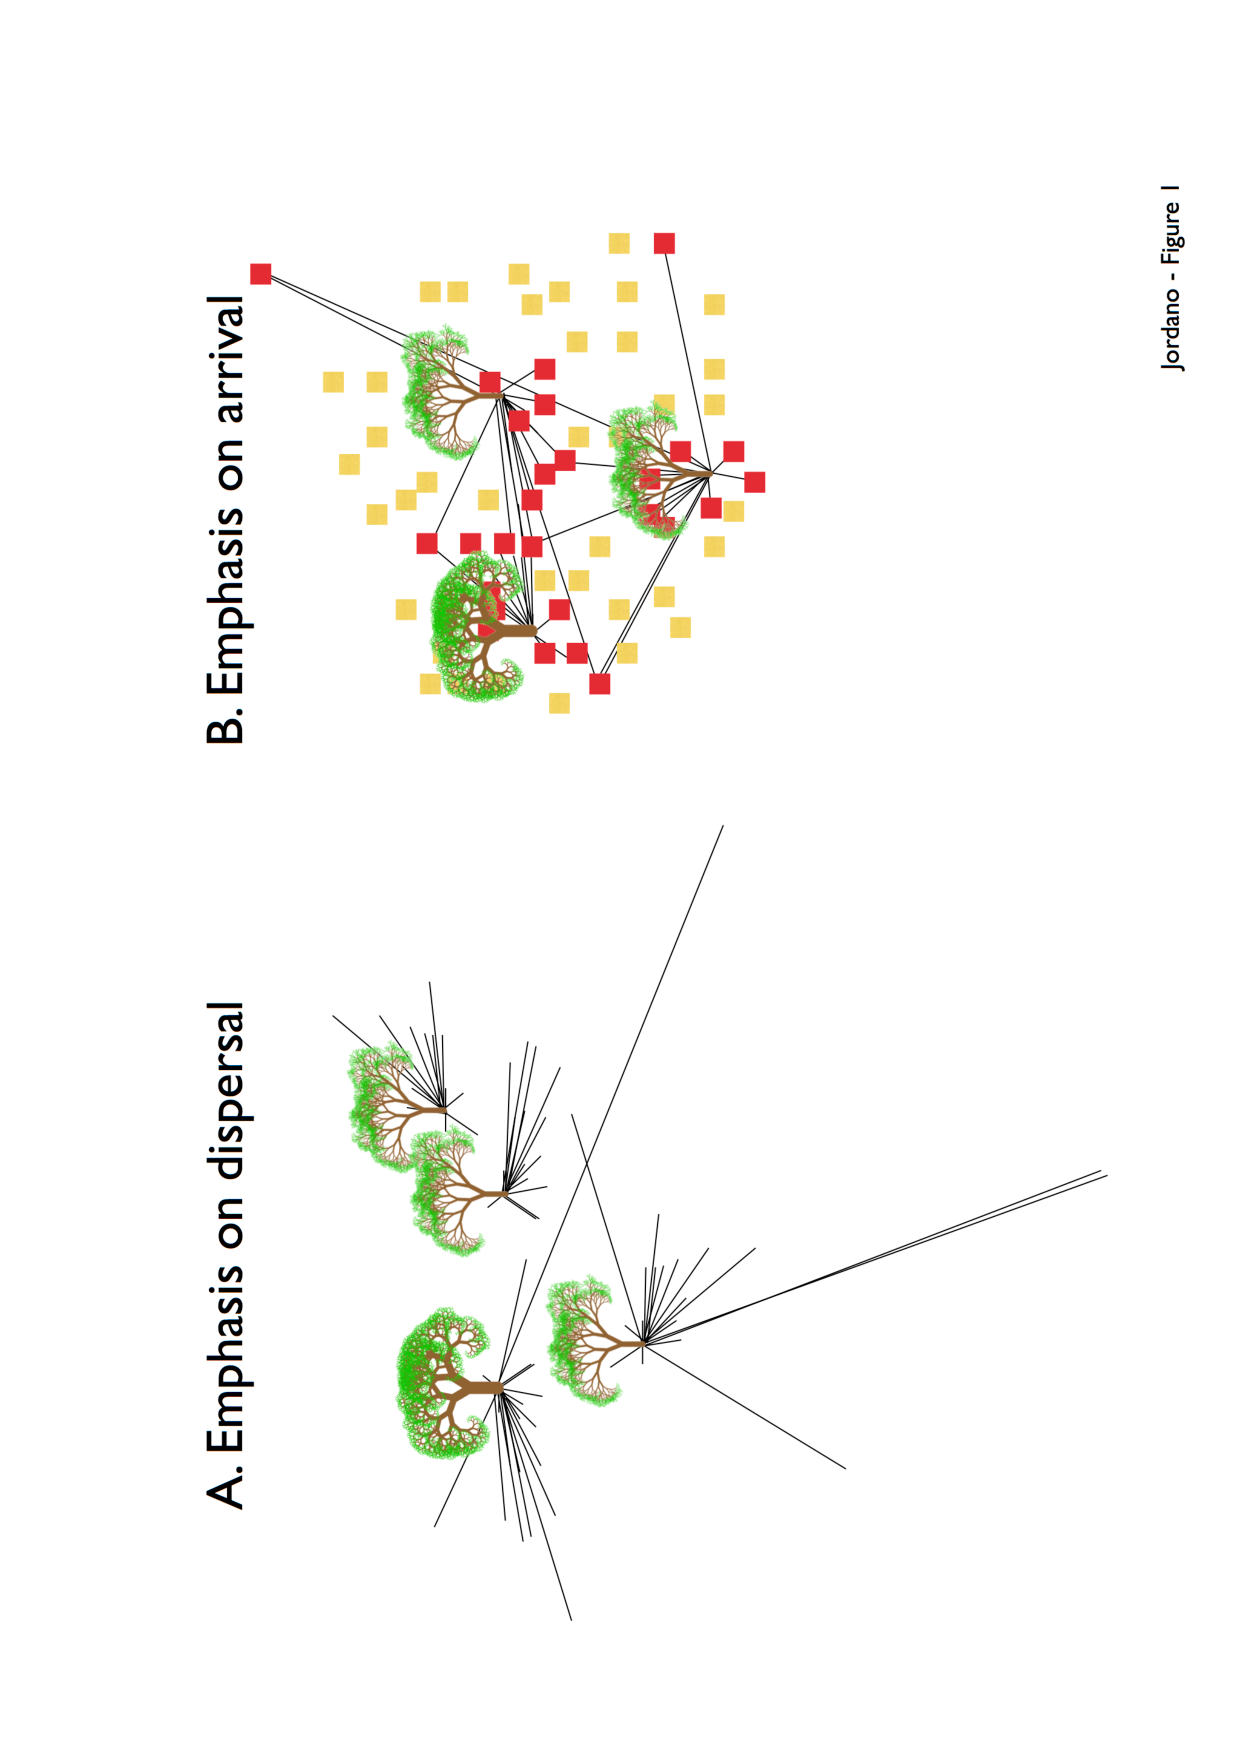
\includegraphics[height=20cm]{Fig1.pdf}}
\caption{Types of dispersal events related to population limits and genetic neigborhood size. The grey area depicts the breeding unit area. Depending on its size it may overlap with neighbour populations (bottom) or be much smaller than the population limits (top). Consequently, strcit sense LDD events $LDD_{SS}$ should be considered those beyond both the ecological and breeding unit area limits (top). LDD events within a local population ($LDD_{loc}$) can occur when propagules disperse beyond the local limits of the reeding unit area. Propagules exiting the population ($LDD_{neigh}$ but moving within the breeding unit area should not be considered strict sense LDD events. Short distance dispersal events are those occurring within the limits of both the population and breeding unit area $SDD_{loc}$.}
\end{figure}
%----------------------------------------------------------------------------

\end{document}

